% FIXME1 divide this file into separate ones...
\chapterold{Working with floating point numbers using SIMD}

\label{floating_SIMD}
\myindex{IEEE 754}
\myindex{SIMD}
\myindex{SSE}
\myindex{SSE2}

Of course, the \ac{FPU} has remained in x86-compatible processors when the \ac{SIMD} extensions were added.

The \ac{SIMD} extensions (SSE2) offer an easier way to work with floating-point numbers.

The number format remains the same (IEEE 754).

\myindex{x86-64}
So, modern compilers (including those generating
for x86-64) usually use \ac{SIMD} instructions instead of FPU ones.

It can be said that it's good news, because it's easier to work with them.

We are going to reuse the examples from the FPU section here: \myref{sec:FPU}.

\sectionold{Simple example}

\lstinputlisting{patterns/12_FPU/1_simple/simple.c}

\subsectionold{x64}

\lstinputlisting[caption=\Optimizing MSVC 2012 x64]{patterns/205_floating_SIMD/simple_MSVC_2012_x64_Ox.asm}

The input floating point values are passed in the \XMM{0}-\XMM{3} registers,
all the rest---via the stack
\footnote{\href{http://go.yurichev.com/17263}{MSDN: Parameter Passing}}.

$a$ is passed in \XMM{0}, $b$\EMDASH{}via \XMM{1}.

The XMM-registers are 128-bit (as we know from the section about \ac{SIMD}: \myref{SIMD_x86}), 
but the \Tdouble values are 64 bit, so only lower register half is used.

\myindex{x86!\Instructions!DIVSD}
\TT{DIVSD} is an SSE-instruction that stands for 
\q{Divide Scalar Double-Precision Floating-Point Values}, 
it just divides
one value of type \Tdouble by another, stored in the lower halves of operands.

The constants are encoded by compiler in IEEE 754 format.

\myindex{x86!\Instructions!MULSD}
\myindex{x86!\Instructions!ADDSD}
\TT{MULSD} and \TT{ADDSD} work just as the same, but do multiplication and addition.

The result of the function's execution in type \Tdouble is left in the in \XMM{0} register.\\
\\
That is how non-optimizing MSVC works:

\lstinputlisting[caption=MSVC 2012 x64]{patterns/205_floating_SIMD/simple_MSVC_2012_x64.asm}

\myindex{Shadow space}
Slightly redundant. 
The input arguments are saved in the \q{shadow space} (\myref{shadow_space}), 
but only their lower register halves, i.e., only 64-bit values of type \Tdouble.
GCC produces the same code.

\subsectionold{x86}

Let's also compile this example for x86. Despite the fact it's generating for x86, MSVC 2012 uses SSE2 instructions:

\lstinputlisting[caption=\NonOptimizing MSVC 2012 x86]{patterns/205_floating_SIMD/simple_MSVC_2012_x86.asm}

\lstinputlisting[caption=\Optimizing MSVC 2012 x86]{patterns/205_floating_SIMD/simple_MSVC_2012_x86_Ox.asm}

It's almost the same code, however, there are some differences related to calling conventions:
1) the arguments are passed not in XMM registers, but in the stack, like in the FPU examples (\myref{sec:FPU});
2) the result of the function is returned in \ST{0} --- in order to do so, it's copied
(through local variable \TT{tv}) from one of the XMM registers to \ST{0}.

\clearpage
Let's try the optimized example in \olly:

\begin{figure}[H]
\centering
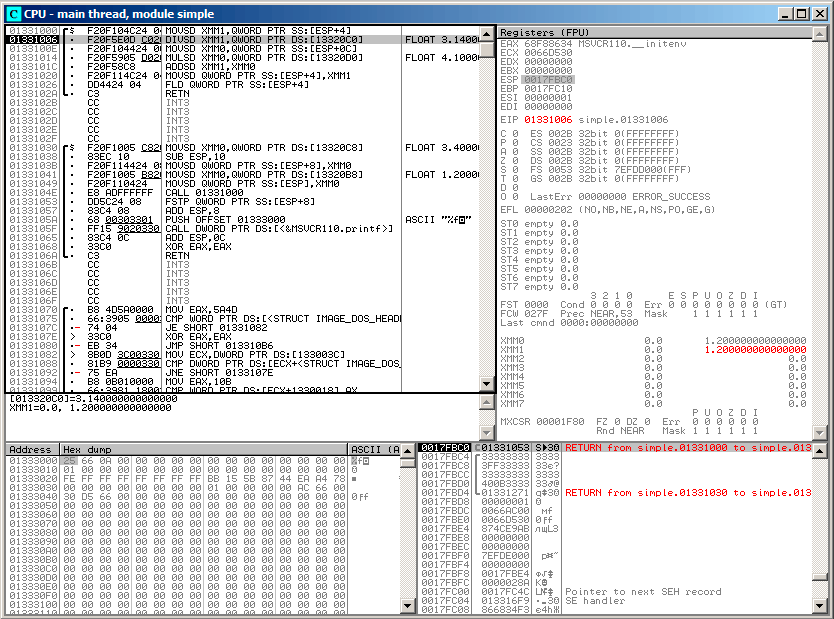
\includegraphics[scale=\FigScale]{patterns/205_floating_SIMD/simple_olly1.png}
\caption{\olly: \TT{MOVSD} loads the value of $a$ into \XMM{1}}
\label{fig:FPU_SIMD_simple_olly1}
\end{figure}

\clearpage
\begin{figure}[H]
\centering
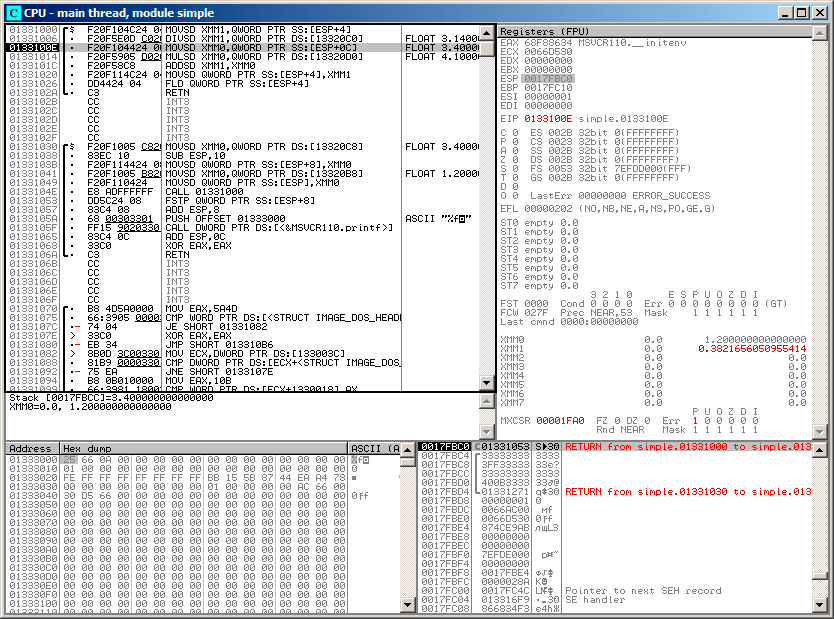
\includegraphics[scale=\FigScale]{patterns/205_floating_SIMD/simple_olly2.png}
\caption{\olly: \TT{DIVSD} calculated \gls{quotient} 
and stored it in \XMM{1}}
\label{fig:FPU_SIMD_simple_olly2}
\end{figure}

\clearpage
\begin{figure}[H]
\centering
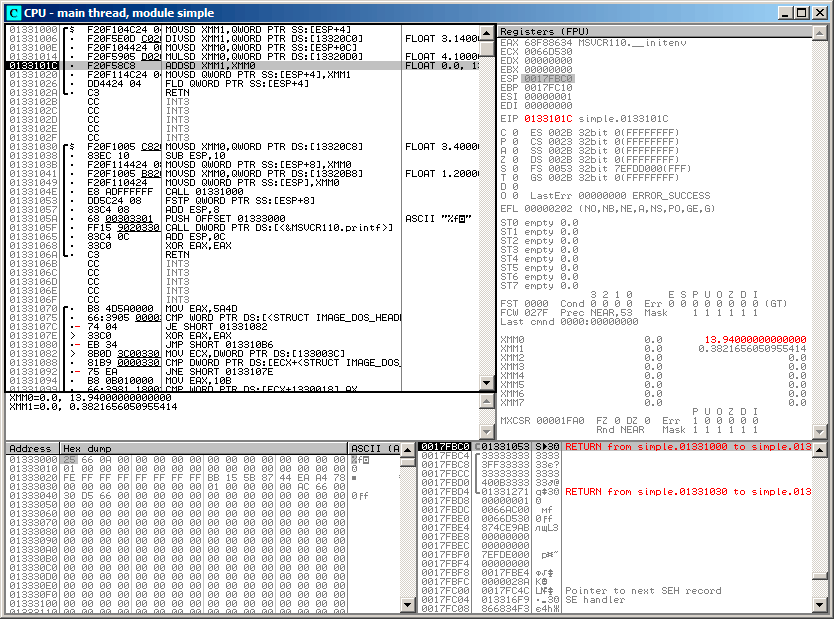
\includegraphics[scale=\FigScale]{patterns/205_floating_SIMD/simple_olly3.png}
\caption{\olly: \TT{MULSD} calculated \gls{product} and stored it
in \XMM{0}}
\label{fig:FPU_SIMD_simple_olly3}
\end{figure}

\clearpage
\begin{figure}[H]
\centering
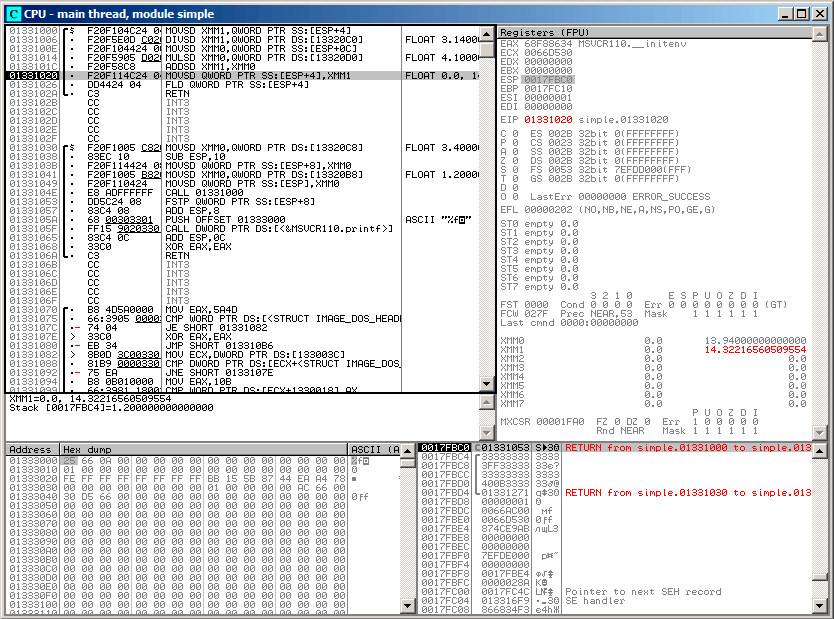
\includegraphics[scale=\FigScale]{patterns/205_floating_SIMD/simple_olly4.png}
\caption{\olly: \TT{ADDSD} adds value in \XMM{0} to \XMM{1}}
\label{fig:FPU_SIMD_simple_olly4}
\end{figure}

\clearpage
\begin{figure}[H]
\centering
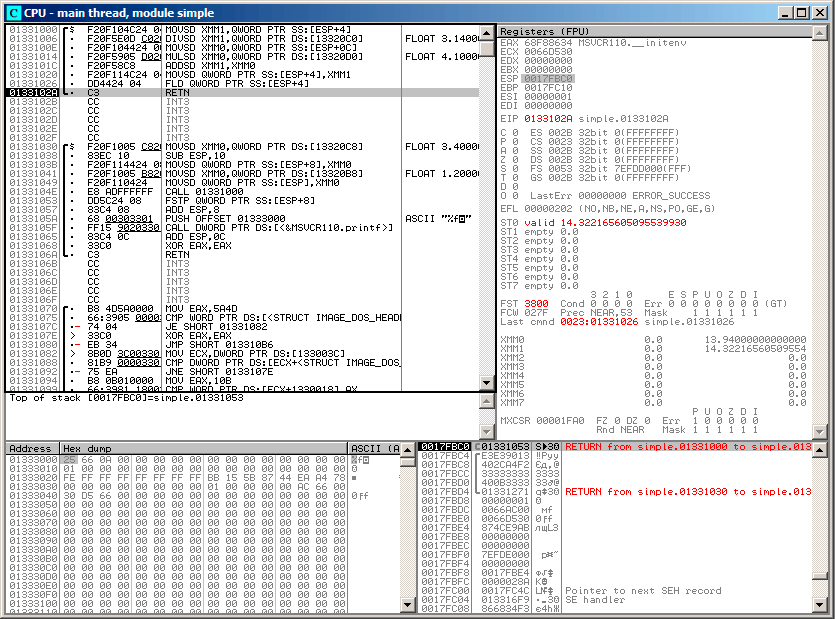
\includegraphics[scale=\FigScale]{patterns/205_floating_SIMD/simple_olly5.png}
\caption{\olly: \FLD left function result in \ST{0}}
\label{fig:FPU_SIMD_simple_olly5}
\end{figure}

We see that \olly shows the XMM registers as pairs of \Tdouble numbers,
but only the \IT{lower} part is used.

Apparently, \olly shows them in that format because the SSE2 instructions (suffixed with \TT{-SD}) 
are executed right now.

But of course, it's possible to switch the register format and to see their contents as
4 \Tfloat{}-numbers or just as 16 bytes.

\clearpage
\sectionold{Passing floating point number via arguments}

\lstinputlisting{patterns/12_FPU/2_passing_floats/pow.c}

They are passed in the lower halves
of the \XMM{0}-\XMM{3} registers.

\lstinputlisting[caption=\Optimizing MSVC 2012 x64]{patterns/205_floating_SIMD/pow_MSVC_2012_x64_Ox.asm}

\myindex{x86!\Instructions!MOVSD}
\myindex{x86!\Instructions!MOVSDX}
There is no \TT{MOVSDX} instruction in Intel and AMD  manuals (\myref{x86_manuals}), there it is called just \TT{MOVSD}.
So there are two instructions sharing the same name in x86 (about the other see: \myref{REP_MOVSx}).
Apparently, Microsoft developers wanted to get rid of the mess, so they renamed it to \TT{MOVSDX}.
It just loads a value into the lower half of a XMM register.

\TT{pow()} takes arguments from \XMM{0} and \XMM{1}, and returns result in \XMM{0}.
It is then moved to \RDX for \printf. 
Why? 
Maybe because 
\printf\EMDASH{}is a variable arguments function?

\lstinputlisting[caption=\Optimizing GCC 4.4.6 x64]{patterns/205_floating_SIMD/pow_GCC446_x64_O3_EN.s}

GCC generates clearer output. 
The value for \printf is passed in \XMM{0}. 
By the way, here is a case when 1 is written into \EAX
for \printf ---this implies that one argument will be passed in vector registers,
just as the standard requires \SysVABI.

\sectionold{Comparison example}

\lstinputlisting{patterns/12_FPU/3_comparison/d_max.c}

\subsectionold{x64}

\lstinputlisting[caption=\Optimizing MSVC 2012 x64]{patterns/205_floating_SIMD/d_max_MSVC_2012_x64_Ox.asm}

\Optimizing MSVC generates a code very easy to understand.

\myindex{x86!\Instructions!COMISD}
\TT{COMISD} is \q{Compare Scalar Ordered Double-Precision Floating-Point 
Values and Set EFLAGS}. Essentially, that is what it does.\\
\\
\NonOptimizing MSVC generates more redundant code,
but it is still not hard to understand:

\lstinputlisting[caption=MSVC 2012 x64]{patterns/205_floating_SIMD/d_max_MSVC_2012_x64.asm}

\myindex{x86!\Instructions!MAXSD}
However, GCC 4.4.6 
did more optimizations and used the \TT{MAXSD} (\q{Return Maximum Scalar 
Double-Precision Floating-Point Value}) instruction,
which just choose the maximum value!

\lstinputlisting[caption=\Optimizing GCC 4.4.6 x64]{patterns/205_floating_SIMD/d_max_GCC446_x64_O3.s}

\clearpage
\subsectionold{x86}

Let's compile this example in MSVC 2012 with optimization turned on:

\lstinputlisting[caption=\Optimizing MSVC 2012 x86]{patterns/205_floating_SIMD/d_max_MSVC_2012_x86_Ox.asm}

Almost the same, but the values of $a$ and $b$ are taken from the stack and the function result 
is left in \ST{0}.

If we load this example in \olly, 
we can see how the \TT{COMISD} instruction compares values and sets/clears the \CF and \PF flags:

\begin{figure}[H]
\centering
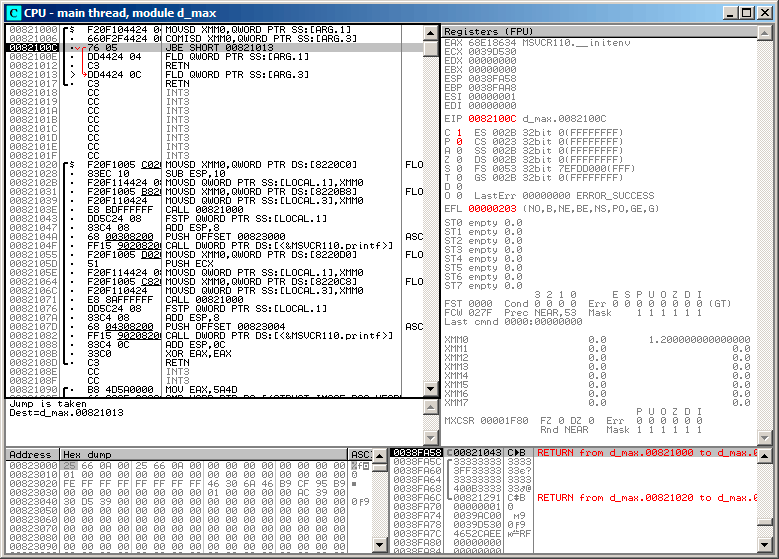
\includegraphics[scale=\FigScale]{patterns/205_floating_SIMD/d_max_olly.png}
\caption{\olly: \TT{COMISD} changed \CF and \PF flags}
\label{fig:FPU_SIMD_d_max_olly}
\end{figure}

\sectionold{Calculating machine epsilon: x64 and SIMD}
\label{machine_epsilon_x64_and_SIMD}

Let's revisit the \q{calculating machine epsilon} example for \Tdouble \lstref{machine_epsilon_double_c}.

Now we compile it for x64:

\lstinputlisting[caption=\Optimizing MSVC 2012 x64]{patterns/205_floating_SIMD/epsilon_double_MSVC_2012_x64_Ox.asm}

There is no way to add 1 to a value in 128-bit XMM register, so it must be placed into memory.

There is, however, the ADDSD instruction (\IT{Add Scalar Double-Precision Floating-Point Values}) 
which can add a value to the lowest 64-bit half of a XMM register while ignoring the higher one, 
but MSVC 2012 probably is not that good yet
\footnote{As an exercise, you may try to rework this code to 
eliminate the usage of the local stack.}.

Nevertheless, the value is then reloaded to a XMM register and subtraction occurs.
SUBSD is \q{Subtract Scalar Double-Precision Floating-Point Values}, 

i.e., it operates on the lower 64-bit part of 128-bit XMM register.
The result is returned in the XMM0 register.

\section{Pseudo-random number generator example revisited}
\label{FPU_PRNG_SIMD}

Let's revisit \q{pseudo-random number generator example} example \lstref{FPU_PRNG}.

If we compile this in MSVC 2012, it will use the SIMD instructions for the FPU.

\lstinputlisting[caption=\Optimizing MSVC 2012]{patterns/205_floating_SIMD/FPU_PRNG/MSVC2012_Ox_Ob0_EN.asm}

% FIXME1 rewrite!

All instructions have the -SS suffix, which stands for \q{Scalar Single}.

\q{Scalar} implies that only one value is stored in the register.

\q{Single} stands for \Tfloat data type.



\sectionold{Summary}

Only the lower half of XMM registers is used in all examples here, 
to store number in IEEE 754 format.

Essentially, all instructions prefixed by 
\TT{-SD} (\q{Scalar Double-Precision})\EMDASH{}are instructions working with floating point numbers
in IEEE 754 format, stored in the lower 64-bit half of a XMM register.

And it is easier than in the FPU, probably because the SIMD extensions 
were evolved in a less chaotic way than the FPU ones in the past.
The stack register model is not used.

\myindex{x86!\Instructions!ADDSS}
\myindex{x86!\Instructions!MOVSS}
\myindex{x86!\Instructions!COMISS}
% TODO1: do this!
If you would try to replace \Tdouble with \Tfloat

% FIXME1 ... but their -SS versions
in these examples, the same instructions will be used, but prefixed with \TT{-SS} 
(\q{Scalar Single-Precision}), for example, \TT{MOVSS}, \TT{COMISS}, \TT{ADDSS}, \etc{}.

\q{Scalar} 
implies that the SIMD register containing only one value instead of several.

Instructions working with several values in a register simultaneously have \q{Packed} in their name.

Needless to say, the SSE2 instructions work with 64-bit IEEE 754 numbers (\Tdouble),
while the internal representation of the floating-point numbers in FPU is 80-bit numbers.

Hence, the FPU may produce less round-off errors and as a consequence, FPU may give more precise
calculation results.
